\documentclass{article} 
\UseRawInputEncoding
\usepackage[utf8]{inputenc}
\usepackage[T1]{fontenc}
\usepackage{selinput}
\usepackage[spanish]{babel}
\usepackage{hyphenat}
\usepackage{graphicx} 
\usepackage{subcaption}
\usepackage{hyperref}
\usepackage{listings}
\usepackage{xcolor}
\usepackage{float}
\usepackage[a4paper, total={6in, 9in}]{geometry}
\SelectInputMappings{%
  eacute={é},
}

\definecolor{codegreen}{rgb}{0,0.6,0}
\definecolor{codegray}{rgb}{0.5,0.5,0.5}
\definecolor{codepurple}{rgb}{0.58,0,0.82}
\definecolor{backcolour}{rgb}{0.95,0.95,0.92}

\lstdefinestyle{mystyle}{
    backgroundcolor=\color{backcolour},
    commentstyle=\color{codegreen},
    keywordstyle=\color{blue},
    numberstyle=\tiny\color{codegray},
    stringstyle=\color{codepurple},
    basicstyle=\ttfamily\footnotesize,
    breakatwhitespace=false,
    breaklines=true,
    captionpos=b,
    keepspaces=true,
    numbers=left,
    numbersep=5pt,
    showspaces=false,
    showstringspaces=false,
    showtabs=false,
    tabsize=2
}

\lstdefinelanguage{CSS}{
  keywords={color,background-image:,margin,padding,font,weight,display,position,top,left,right,bottom,list,style,border,size,white,space,min,width, transition:, transform:, transition-property, transition-duration, transition-timing-function},	
  sensitive=true,
  morecomment=[l]{//},
  morecomment=[s]{/*}{*/},
  morestring=[b]',
  morestring=[b]",
  alsoletter={:},
  alsodigit={-}
}
\lstset{style=mystyle}
\title{Carpeta de Campo BIAS}

\date{}

\begin{document}

\maketitle

\vspace{1cm} 

\textbf{Integrantes del Proyecto:} 

\begin{itemize}
    \item Adell, Nicolas Fabian
    \item De Blasi, Luca
    \item Diaz Melion, Danilo Sebastian
    \item Gil Soria, Ian Lucas
    \item Montenegro, Luciano Nahuel
    \item Sojka, Santiago Alejandro
\end{itemize}

\newpage







\begin{center}
    \section{Marzo de 2024}
\end{center}

Inicio de anteproyecto e investigación sobre la utilización de MATLAB, Python y cómo vincular el Neurosky Mindwave Mobile 2 a una computadora o celular. Decisión de elección de microcontrolador y hardware a utilizar.

\begin{center}
    \href{https://theses.hal.science/tel-04011453v1/document}{https://theses.hal.science/tel-04011453v1/document}
\end{center}

Realización y testeo del código para poder mover la silla de ruedas mediante un joystick.
Investigación sobre los posibles materiales a utilizar en el proyecto ya existentes en la escuela. Hemos visto las posibles sillas de ruedas a utilizar en el proyecto.
Investigación del sensor ultrasónico a utilizar en el proyecto.

Hemos empezado a realizar la programación de los motores y la programación del ultrasonido y se han probado en protoboard, probando que funcionan. También se han hecho ciertas modificaciones al anteproyecto, y se ha empezado a hacer el diagrama temporal. 

\begin{figure}[H]
    \centering
    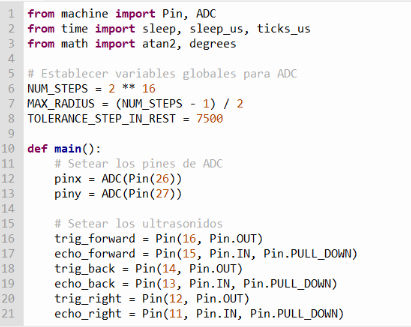
\includegraphics[width=0.75\linewidth]{Imagenes//Marzo/ProgramacionMotores.png}
\end{figure}


Hemos hecho el logo del proyecto, hemos encontrado las baterías necesarias para poder mover la silla de ruedas, discutimos, tanto entre nosotros como con otros profesores, sobre la utilización de 1 o 2 motores, discutimos sobre los drivers y el puente H.

\begin{figure}[H]
    \centering
    
\includegraphics[width=0.75\linewidth]{Imagenes//Marzo/LogoBIAS.png}
\end{figure}

\newpage

En el día de la fecha hemos creado la cuenta  de la red social instagram junto al mail mismo del proyecto.

\begin{figure}[H]
    \centering
    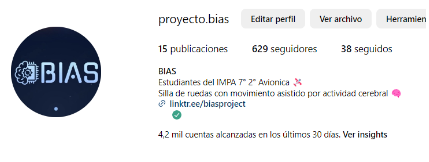
\includegraphics[width=0.75\linewidth]{Imagenes//Marzo/InstagramBias.png}
\end{figure}


Hemos realizado el esquemático junto al diseño del pcb del sistema de emergencias, por lo que quedaría imprimirlo y ya ir armando la placa.

\begin{figure}[H]
    \centering
    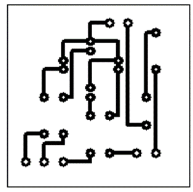
\includegraphics[width=0.45\linewidth]{Imagenes//Marzo/SistemadeEmergencias.png}
\end{figure}

Investigamos la datasheet del driver del motor, empezamos a investigar el circuito interno y las posibilidades a la hora de manejar el motor.

\begin{figure}[H]
    \centering
    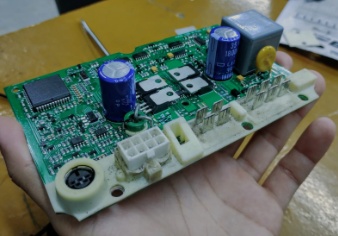
\includegraphics[width=0.65\linewidth]{Imagenes//Marzo/DriverFoto.png}
\end{figure}

\newpage

Empezamos a desarrollar el programa para conectar el Neurosky a un módulo HC-05.

\begin{figure}[H]
    \centering
    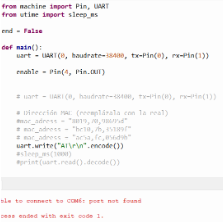
\includegraphics[width=0.65\linewidth]{Imagenes//Marzo/ProgramaNeurosky.png}
\end{figure}


\begin{center}
    \section{Abril de 2024}
\end{center}

Hemos empezado a organizarnos con la plataforma trello para tener buena percepción sobre las tareas a realizar.

\begin{figure}[H]
    \centering
    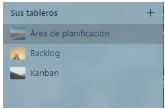
\includegraphics[width=0.5\linewidth]{Imagenes//Abril/Trello.png}
\end{figure}


\newpage

Estuvimos buscando la forma de conectar el Neurosky a la computadora a través de bluetooth, y terminamos optando por seguir con el HC-05, ya que no se conecta directamente y las versiones no son compatibles.



\begin{figure}[H]
    \centering
    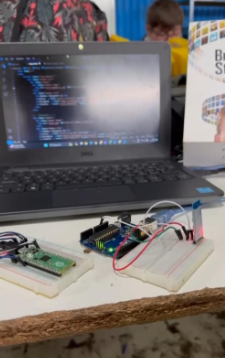
\includegraphics[width=0.35\linewidth]{Imagenes//Abril/ProgramacionNeurosky.png}
\end{figure}

Hicimos las imágenes que vamos a publicar al Instagram a la hora de que verifiquen el LinkedIn, seguimos desarrollando el programa para usar el módulo bluetooth (HC-05), empezamos a hacer un plano de la silla de ruedas para hacer las modificaciones de la estructura que tengamos que hacer.

\begin{figure}[H]
    \centering
    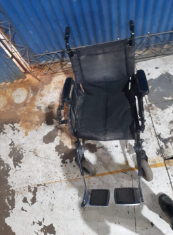
\includegraphics[width=0.45\linewidth]{Imagenes//Abril/SilladeRuedas.png}
\end{figure}

\newpage

Se consiguió con éxito poder establecer la conexión Bluetooth del HC05 a una computadora 

\begin{figure}[H]
    \centering
    \includegraphics[width=0.5\linewidth]{Imagenes//Abril/HC05.png}
\end{figure}

Cargamos las baterías y empezamos a probar los motores junto al driver, investigamos sobre otras opciones para reemplazar al Neurosky, ya que no hay forma de hacerlos vincular..

\begin{figure}[H]
    \centering
    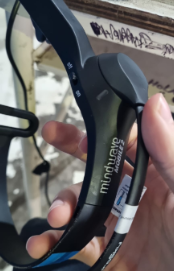
\includegraphics[width=0.5\linewidth]{Imagenes//Abril/Neurosky.png}
\end{figure}

\newpage

Desarrollamos la página del proyecto, creamos el GitHub donde estará todo tipo de documento y código relacionado al proyecto y una cuenta de TikTok.

\begin{figure}[H]
    \centering
    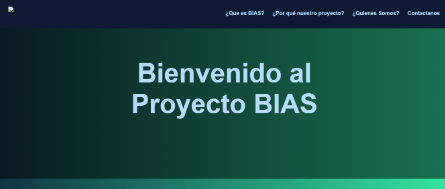
\includegraphics[width=0.95\linewidth]{Imagenes//Abril/PaginaWeb.png}
\end{figure}

Seguimos con la programación del Neurosky Mobile Mindwave 2, además de crear publicaciones para difundirnos por Instagram.

\begin{figure}[H]
    \centering
    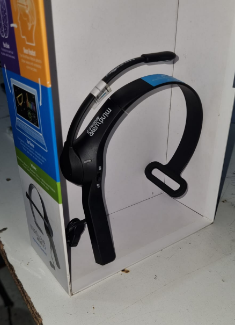
\includegraphics[width=0.5\linewidth]{Imagenes//Abril/NeuroskyCaja.png}
\end{figure}

\newpage


\begin{center}
    \section{Mayo de 2024}
\end{center}






Probamos conectar el Neurosky con Arduino pero sigue sin funcionar. Por eso buscamos otras alternativas para el EEG, ya que debido a los intentos reiterados no funciona.

\begin{figure}[H]
    \centering
    \includegraphics[width=0.3\linewidth]{Imagenes//Mayo/HC05.png}
\end{figure}



Se investiga el driver si puede funcionar y si es viable utilizarlo o hacer el propio.

\begin{figure}[H]
    \centering
    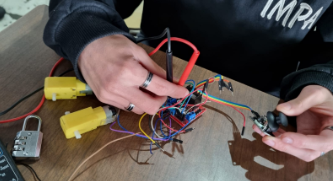
\includegraphics[width=0.75\linewidth]{Imagenes//Mayo/Servos.png}
\end{figure}

\newpage

Fuimos a la radio en Solano a hablar del proyecto. Nos contactamos con la radio FM Sur.

\begin{figure}[H]
    \centering
    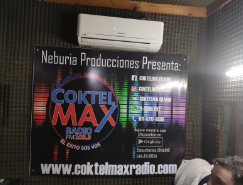
\includegraphics[width=0.5\linewidth]{Imagenes//Mayo/RadioCoktel.png}
\end{figure}


Probamos el driver y el motor originales que venían con la silla de ruedas. Se realiza un informe sobre el Driver ya que el mismo no funciona.

\begin{figure}[H]
    \centering
    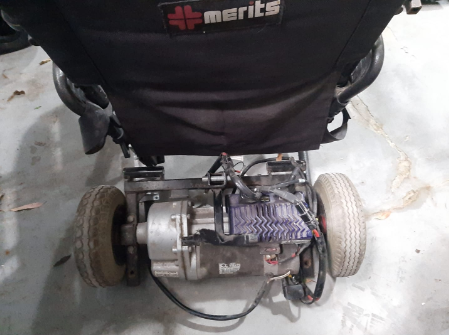
\includegraphics[width=0.55\linewidth]{Imagenes//Mayo/SillaMotor.png}
\end{figure}

Se realizó el plano de la silla de ruedas en Autocad. Se busca la forma de diseño del Driver. Nos contactamos con sponsors para darnos difusión. Organizamos el Trello.

\begin{figure}[H]
    \centering
    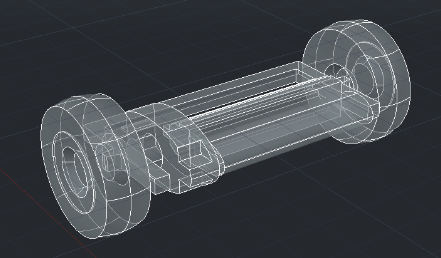
\includegraphics[width=0.55\linewidth]{Imagenes//Mayo/MotorModelo3D.png}
\end{figure}


\newpage

Tuvimos la entrevista radial en FM Sur. Se realiza el reel n.° 3. Se continúa con el plano de la silla. Se organiza el Github. Se buscan alternativas al Neurosky. 

\begin{figure}[H]
    \centering
    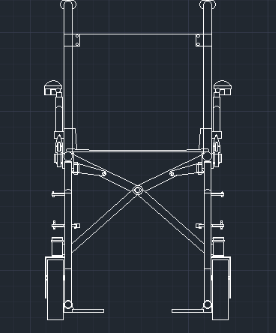
\includegraphics[width=0.45\linewidth]{Imagenes//Mayo/SillaModelo3D.png}
\end{figure}

Se realiza el diseño del driver para el motor. Finalmente se toma el Open BCI como alternativa para realizarla por nosotros mismos debido a los costes de fabricación. Para eso se busca la documentación.

\begin{figure}[H]
    \centering
    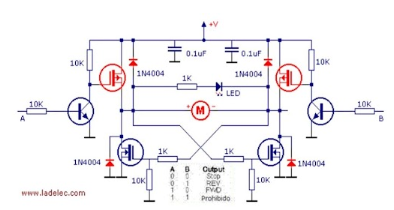
\includegraphics[width=0.55\linewidth]{Imagenes//Mayo/PuenteH.png}
\end{figure}

Nos contactamos con ALAPA, con la Fundación Esteban Bullrich y con la política María Sotolano. Vemos la alternativa del Open BCI

\begin{figure}[H]
    \centering
    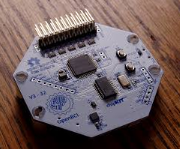
\includegraphics[width=0.35\linewidth]{Imagenes//Mayo/OpenBCI.png}
\end{figure}

\newpage

Realizamos una entrevista para que Clarín haga una nota sobre nosotros.

\begin{figure}[H]
    \centering
    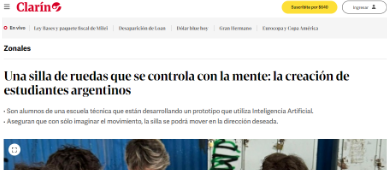
\includegraphics[width=0.75\linewidth]{Imagenes//Mayo/Clarin.png}
\end{figure}




Buscamos de un EEG de reemplazo que tenga un coste aceptable. Elegimos entre el Open BCI y otro circuito. Tomamos el ejemplo de la página siguiente: 

\begin{center}
    \href{https://www.instructables.com/DIY-EEG-and-ECG-Circuit/}{https://www.instructables.com/DIY-EEG-and-ECG-Circuit}
\end{center}

\begin{figure}[H]
    \centering
    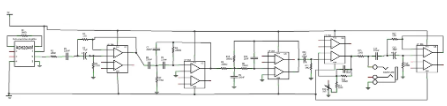
\includegraphics[width=0.85\linewidth]{Imagenes//Mayo/EEG.png}
\end{figure}


Fuimos al Congreso a hablar con la diputada María Sotolano. Logramos asegurar el contacto con la asociación Esteban Bullrich.

\begin{figure}[H]
    \centering
    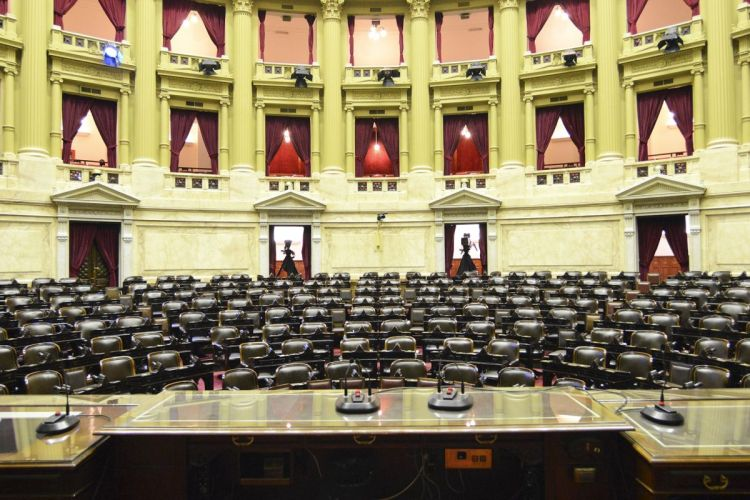
\includegraphics[width=0.75\linewidth]{Imagenes//Mayo/CamaraDiputados.jpg}
\end{figure}

\newpage

TN nos entrevista, por lo que preparamos un stand para presentar en la televisión.

\begin{figure}[H]
    \centering
    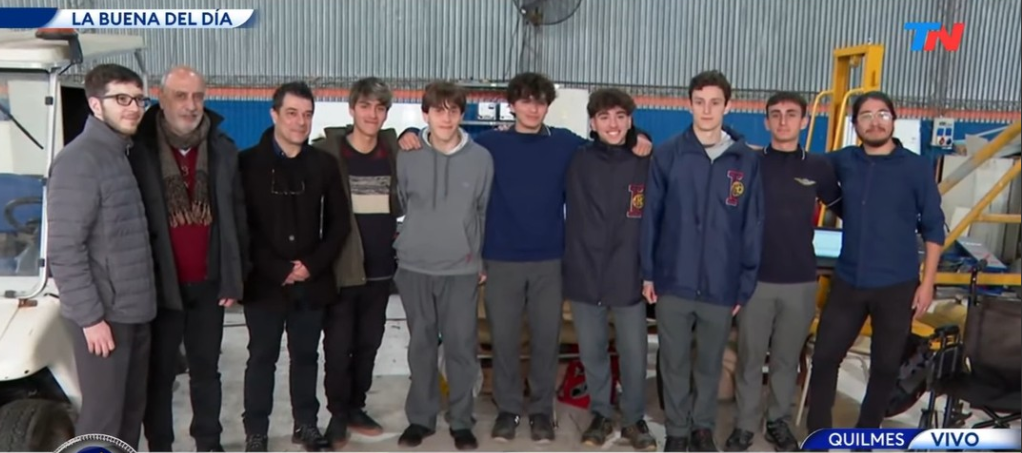
\includegraphics[width=0.95\linewidth]{Imagenes//Mayo/bias.png}
\end{figure}




\begin{center}
    \section{Junio de 2024}
\end{center}



\newpage







\begin{center}
    \section{Julio de 2024}
\end{center}



\newpage















\end{document}
